\documentclass[11pt]{beamer}
\usepackage[OT1]{fontenc}
\usepackage[utf8x]{inputenc}
\usepackage[frenchb]{babel}
%\usepackage[dvipsnames]{xcolor}
\usepackage{xcolor}
\usetheme{PickEM}
\title{D\'eveloppement d'un utilitaire de s\'election de particules observ\'ees au microscope \'electronique}
\subtitle{Greffon Pick\_EM pour ImageJ}
\date{25 Mai 2012}
\author{\textsc{Faux} - \textsc{Héricé} - \textsc{Paysan-Lafosse} - \textsc{Sansen}}
\institute[Universite Bordeaux 1 \& 2] 
{
 Master 1 Bioinformatique \\ Projet de programmation sous la direction de Jean-Christophe \textsc{Taveau} \\ 
 \begin{figure}[h]
  \begin{center}
  
\includegraphics[width=0.25\columnwidth]{logoBdxB.jpeg}
  \hspace{1cm}
  
\includegraphics[width=0.3\columnwidth]{cbmn-1.png}
  \end{center}
 \end{figure}
}

%\AtBeginSection[]{
%  \begin{frame}{Plan}
%  \small \tableofcontents[currentsection, hideothersubsections]
%  \end{frame} 
%} 
 
\begin{document}

\frame{\titlepage}

\section*{Sommaire}

\begin{frame}
  \tableofcontents
\end{frame}

\section{Introduction}

\begin{frame}
	\frametitle{\secname}
	\begin{block}{CBMN}
		Laboratoire de Chimie et Biologie des Membranes et Nanoobjets 
	\end{block}
	\begin{block}{ACMPC}
		\'Equipe Architectures des Complexes Membranaires et Processus Cellulaires
	\end{block}
\end{frame}

\subsection{Contexte}
	\begin{frame}
	\frametitle{\subsecname}
	\begin{columns}
		\begin{column}{6cm}
			\begin{itemize}
			\item Micrographies de complexes protéiques
			\item Utilisation du logiciel ImageJ
			\item Sélection manuelle fastidieuse 
				\begin{itemize}
				\item Chronophage
				\item Accapare un membre de l'équipe	
				\item Répétitive
				\end{itemize}
			\end{itemize}
		\end{column}	
		\begin{column}{6cm}
			\begin{figure}
				\includegraphics[scale=0.08]{BaseEchelle.png}
		
			Exemple de micrographie
			\end{figure}
		\end{column}
	\end{columns}
\end{frame}

\subsection{Objectifs}
\begin{frame}
\frametitle{\subsecname}
	\begin{columns}[t]
		
		\begin{column}{4.5cm}
			\begin{block}{Création d'une interface}
				\begin{itemize}
					\item Facile d'utilisation
					\item Claire et succincte
					\item Récupération des paramètres utilisateurs
				\end{itemize}
			\end{block}
		\end{column}
		\begin{column}{6.5cm}
		    \begin{block}{Implémentation d'algorithmes}
				\begin{itemize}
					\item Automatisation du traitement et de la sélection
					\item Récupération des coordonnées
					\item Images individuelles
				\end{itemize}
			\end{block}
		\end{column}
	\end{columns}
\end{frame}

\section{Analyse}

\subsection{Besoins fonctionnels}

\begin{frame}
\frametitle{\subsecname}
	\begin{columns}[t]
		
		\begin{column}{5cm}
			\begin{block}{Interface}
				\begin{itemize}
					\item Choix entre plusieurs algorithmes
					\item Différente pour chaque algorithme
				\end{itemize}
			\end{block}
			\begin{block}{Algorithmes}
				\begin{itemize}
					\item Sélection automatique
					\item Résultats : tableau de coordonnées (x, y, z) et pile d'images individuelles
				\end{itemize}
			\end{block}
		\end{column}
		\begin{column}{5cm}
			\begin{figure}
				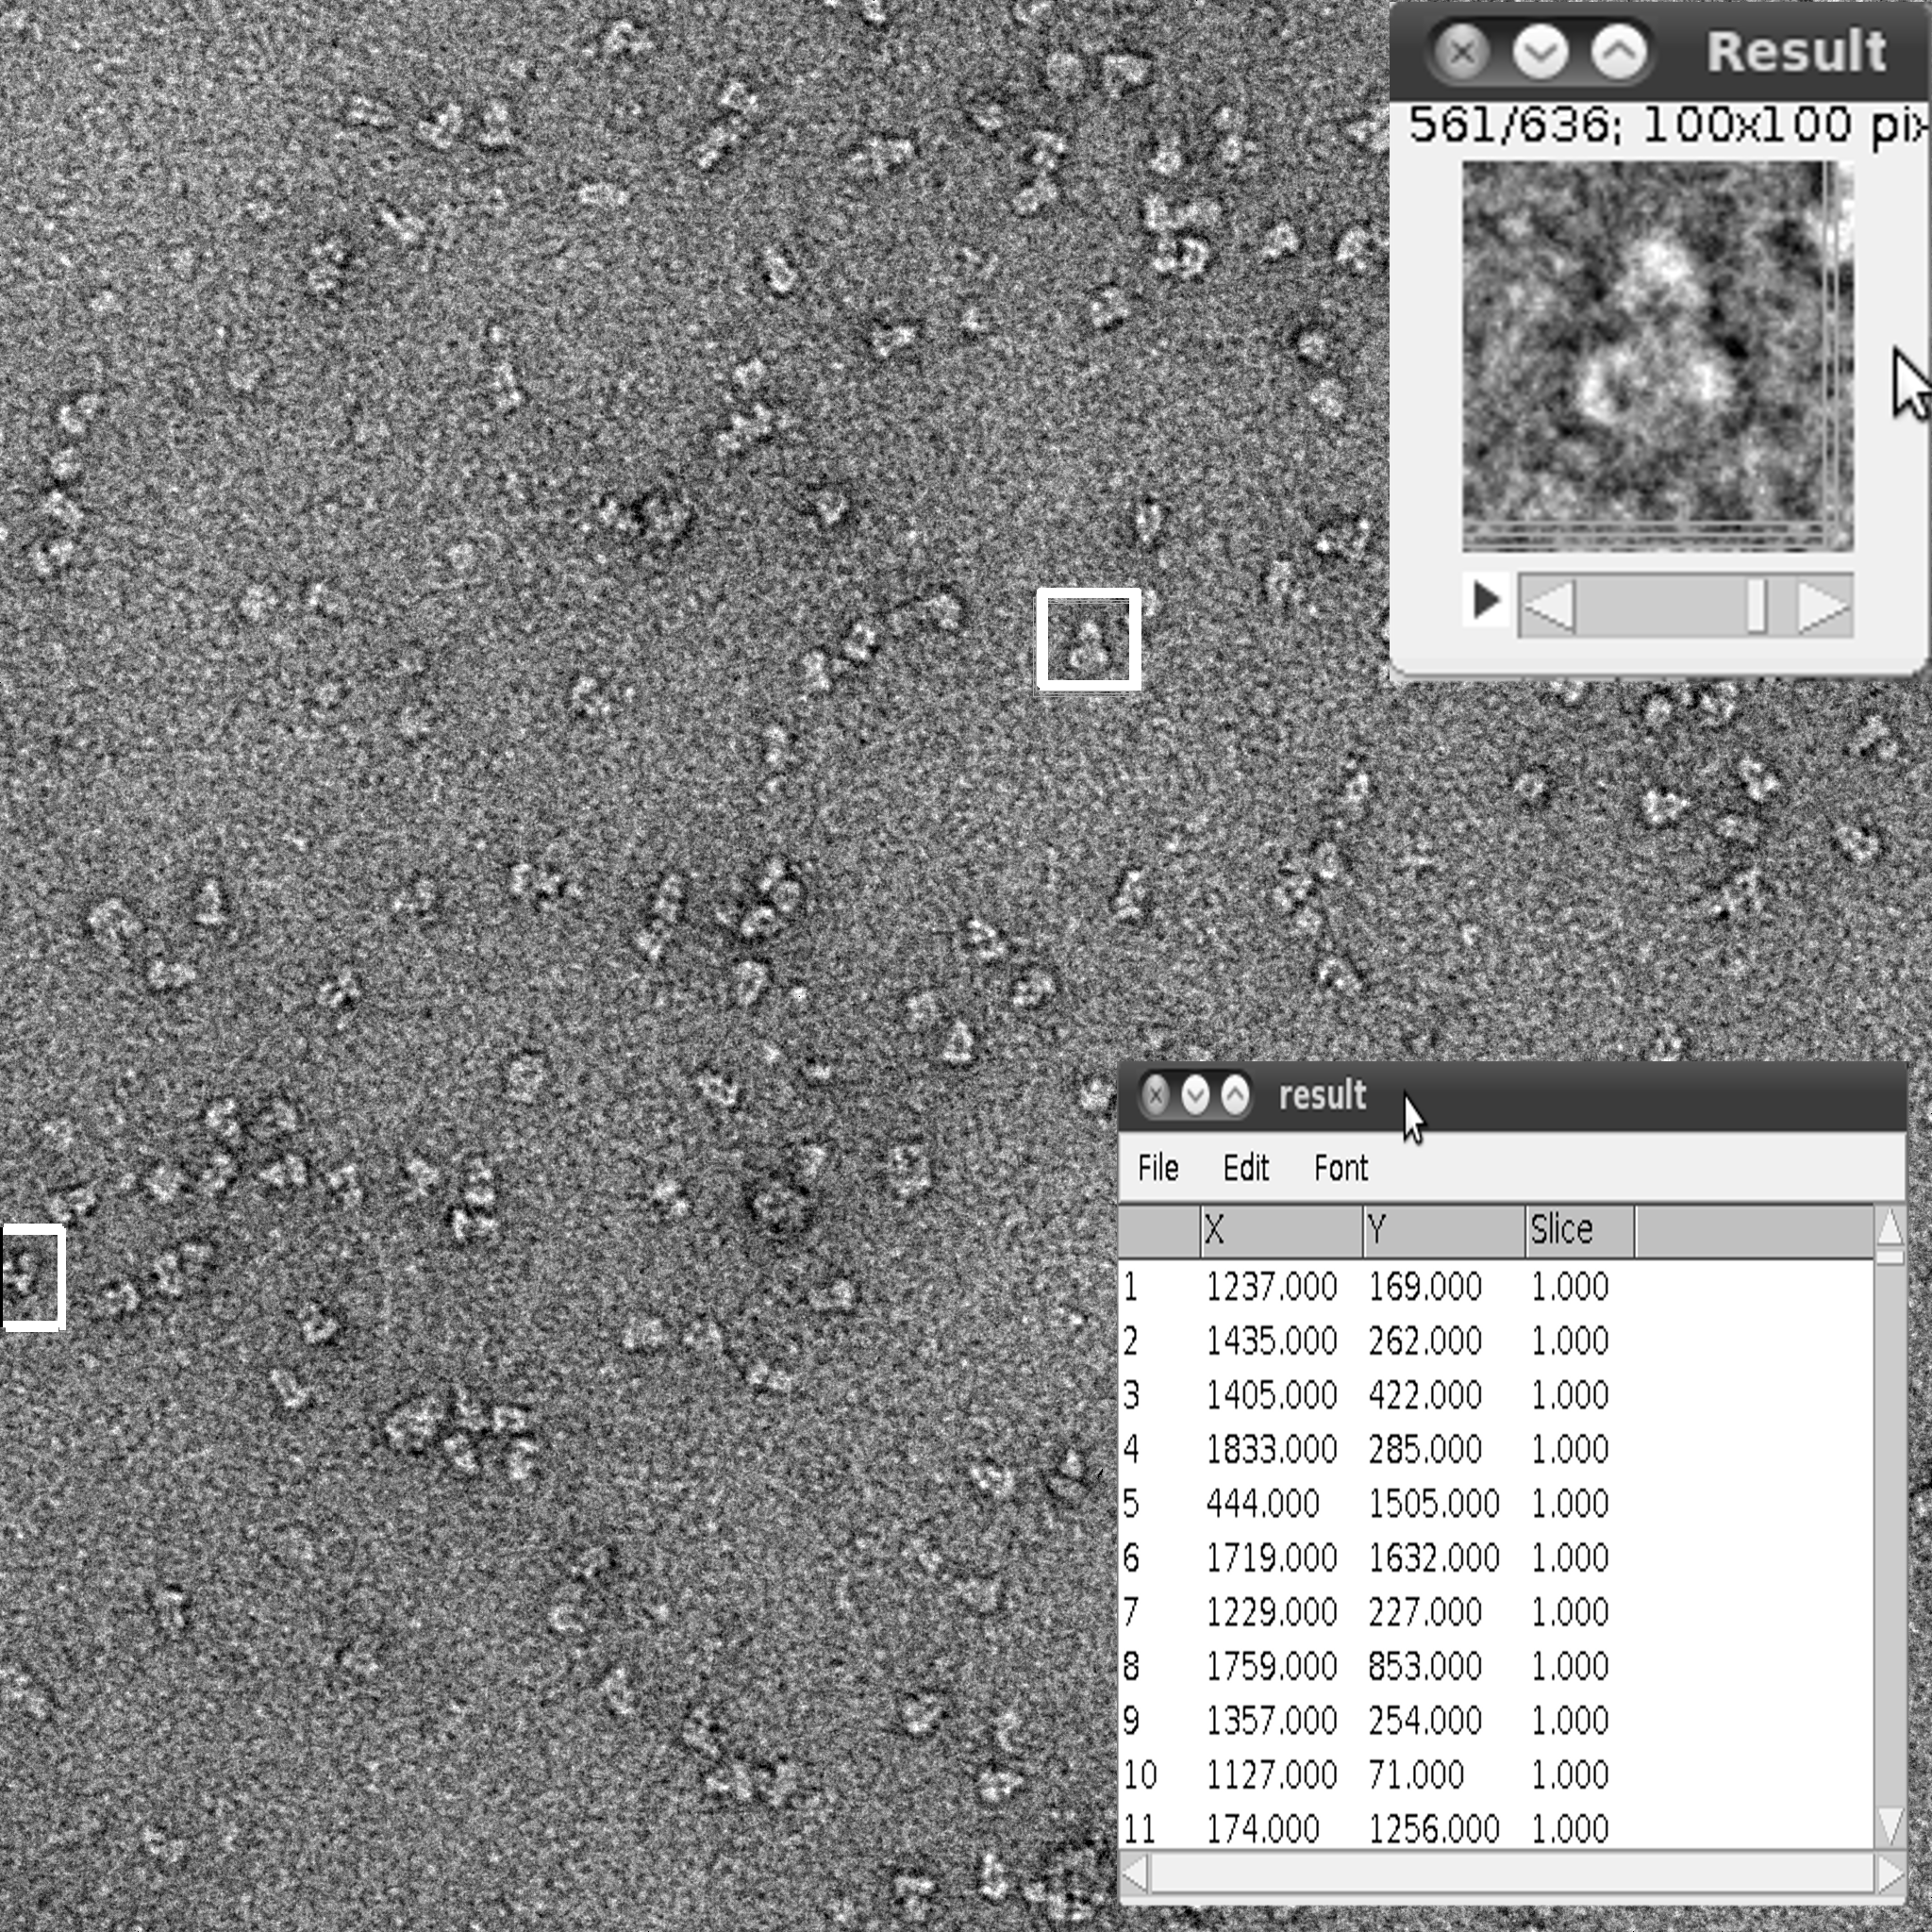
\includegraphics[scale=0.07]{CropResultPickB.png}
				
				Images individuelles et tableau de coordonnées
			\end{figure}
		\end{column}
	\end{columns}	
\end{frame}

\subsection{Besoins non fonctionnels}

\begin{frame}
\frametitle{\subsecname}
	\begin{columns}[t]
		\begin{column}{5cm}
			\begin{block}{Interface}
				\begin{itemize}
					\item Implémentation en Java (AWT ou \textbf{Swing})
					\item Modularité
				\end{itemize}
			\end{block}
		\end{column}
		\begin{column}{5cm}
			\begin{block}{Algorithmes}
				\begin{itemize}
					\item Implémentation en Java
					\item Traitement rapide (grands jeux de données)
					\item Minimiser les étapes intermédiaires
				\end{itemize}
			\end{block}
		\end{column}
	\end{columns}
\end{frame}

\section{Conception - Réalisation}

\subsection{Modularité}

\subsubsection*{Diagramme des classes}
\begin{frame}
\frametitle{\subsecname ~- \subsubsecname}
	\begin{figure}
		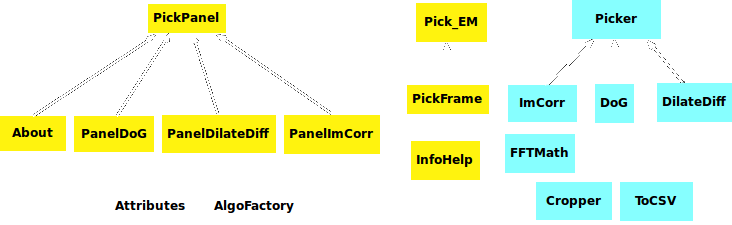
\includegraphics[scale=0.45]{NouvDiag1.png}
	\end{figure}
\end{frame}

\subsubsection*{Patrons de conception}

\begin{frame}
\frametitle{\subsecname ~- \subsubsecname}
\begin{block}{La classe \texttt{Attributes}}
		\emph{HashTable} : couple clé/valeur des paramètres utilisateurs
	\end{block}
	\begin{block}{Singleton}
		%\begin{itemize}
			%\item Sert à n'avoir qu'une seule instance d'une classe à un moment donné
			 Restreint l'instanciation d'une classe à un seul objet
	%	\end{itemize}
	\end{block}
%	hashtable 
	
	\begin{columns}
		\begin{column}{3cm}
			\begin{table}[h]
				\begin{center}
					\begin{tabular}{|c|}
						\hline
						\textbf{Algorithme 1} \\
						\hline
						arg 1 \\
						arg 2 \\
						\hline
					\end{tabular}
				\end{center}
			\end{table}
		\end{column}
		\begin{column}{3cm}
%		\begin{table}[h]
			\begin{table}[h]
				\begin{center}
					\begin{tabular}{|c|}
						\hline
						\textbf{Algorithme 2} \\
						\hline
						arg 1 \\
						arg 2 \\
						param 1 \\
						\hline
					\end{tabular}
				\end{center}
			\end{table}
		\end{column}
	\begin{column}{3cm}
	\begin{table}[h]
		\begin{center}
			\begin{tabular}{|c|}
				\hline
				\textbf{Algorithme 3} \\
				\hline
				param 1 \\
				param 2 \\
				param 3 \\
				param 4 \\
				\hline
			\end{tabular}
		\end{center}
	\end{table}
	\end{column}
	\end{columns}
\end{frame}

\begin{frame}
\frametitle{\subsecname ~- \subsubsecname}
\begin{columns}
	\begin{column}{5cm}
\begin{block}{La classe \texttt{AlgoFactory}}
	\begin{itemize}
	\item actualisation de l'interface
	\item appel aux méthodes de sélection
	\end{itemize}
\end{block}	
\end{column}
	\begin{column}{6.5cm}
\begin{block}{Fabrique de création (\emph{Factory})}
	\begin{itemize}
		\item Classe qui a pour rôle de construire des objets
		\item Seule responsable de la création $/$ distribution de l’objet
	\end{itemize}
\end{block}
\end{column}
	\end{columns}
	
	\begin{figure}
		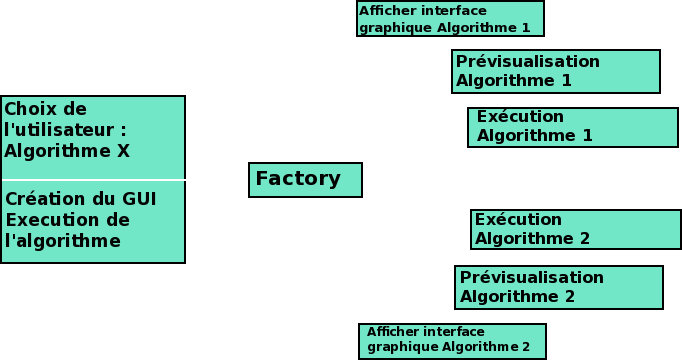
\includegraphics[scale=0.33]{testFabrique.png}
	\end{figure}
\end{frame}
\subsubsection*{Objectif réussi?}
\begin{frame}
\frametitle{\subsecname ~- \subsubsecname}
\begin{block}{Ajout d'un algorithme en 4 étapes :}
	\begin{itemize}
		\item Modification du menu déroulant
		\item Ajout de l'interface et de la méthode de récupération des paramètres 
		\item Création de la classe de sélection en suivant les modèles implémentés
		\item Modification de la classe \texttt{AlgoFactory} pour prendre en compte la nouvelle méthode de sélection
	\end{itemize}
	\end{block}
\end{frame}
\subsection{Interface Graphique (GUI)}
\begin{frame}
\frametitle{\subsecname}\begin{center}

			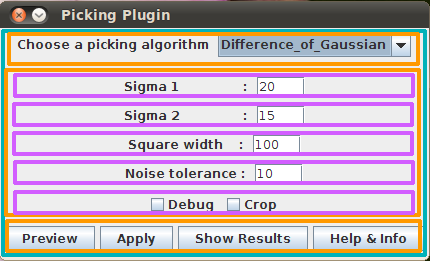
\includegraphics[scale=0.5]{interface2.png}

			Organisation générale de l'interface
\end{center}
\end{frame}

\subsubsection*{Récupération des paramètres utilisateurs}

\begin{frame}
\frametitle{GUI - \subsubsecname}
	%Patrons de Conception : \emph{Factory} et \emph{Singleton}
	\begin{columns}[t]
		\begin{column}{5cm}
			\begin{block}{Choix de l'algorithme}
				\begin{itemize}
					\item JComboBox
				\end{itemize}
			\end{block}
			\vspace*{2cm}
			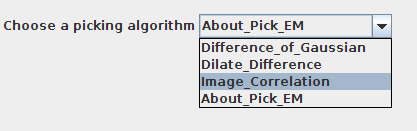
\includegraphics[scale=0.45]{combobx.png}
		\end{column}
		\begin{column}{5cm}
			\begin{block}{Paramètres propres aux algorithmes}
				\begin{itemize}
					\item JTextField
					\item JCheckBox
				\end{itemize}
			\end{block}
			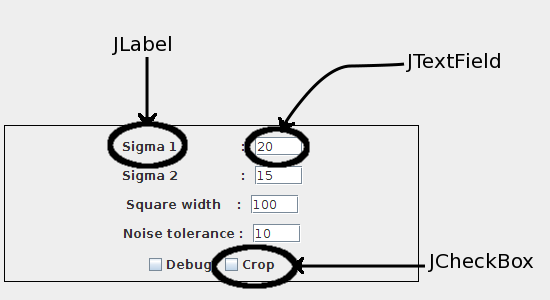
\includegraphics[scale=0.25]{guiObject.png}
		\end{column}
	\end{columns}
\end{frame}

\subsection{Algorithmes}

\subsubsection*{Les algorithmes implémentés}

\begin{frame}
\frametitle{\subsubsecname}
\begin{block}{3 algorithmes implémentés:}
\begin{itemize}
\item Extraction de contours par morphologie mathématique
\item Corrélation croisée d'images
\item Différence de Gaussiennes (DoG)
\end{itemize}
\end{block}
\begin{block}{Schéma général du traitement des images}
\begin{itemize}
\item Pré-traitement (filtrage)
\item Traitement 
\item Post-traitement (tri des résultats)
\end{itemize}
\end{block}
\end{frame}

\begin{frame}
\frametitle{\subsecname ~- Extraction de contours}
\begin{columns}
		\begin{column}{3cm}
			\begin{figure}
				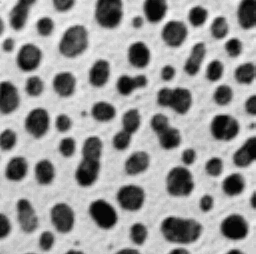
\includegraphics[scale=0.33]{blobs.png}

				Image avant traitement
			\end{figure}
		\end{column}
		\begin{column}{3cm}
			\begin{figure}
				
\includegraphics[scale=0.33]{blobDilateDiffResult.png}

				Image résultante
			\end{figure}
		\end{column}
		\begin{column}{3cm}
			\begin{figure}
				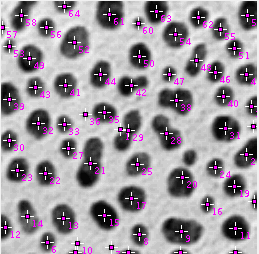
\includegraphics[scale=0.33]{blobDilate.png}

				Image avec les sélections
			\end{figure}
		\end{column}
	\end{columns}
\end{frame}

\begin{frame}
\frametitle{\subsecname ~- Corrélation croisée d'images}
	\begin{columns}
		\begin{column}{5cm}
			\begin{figure}
				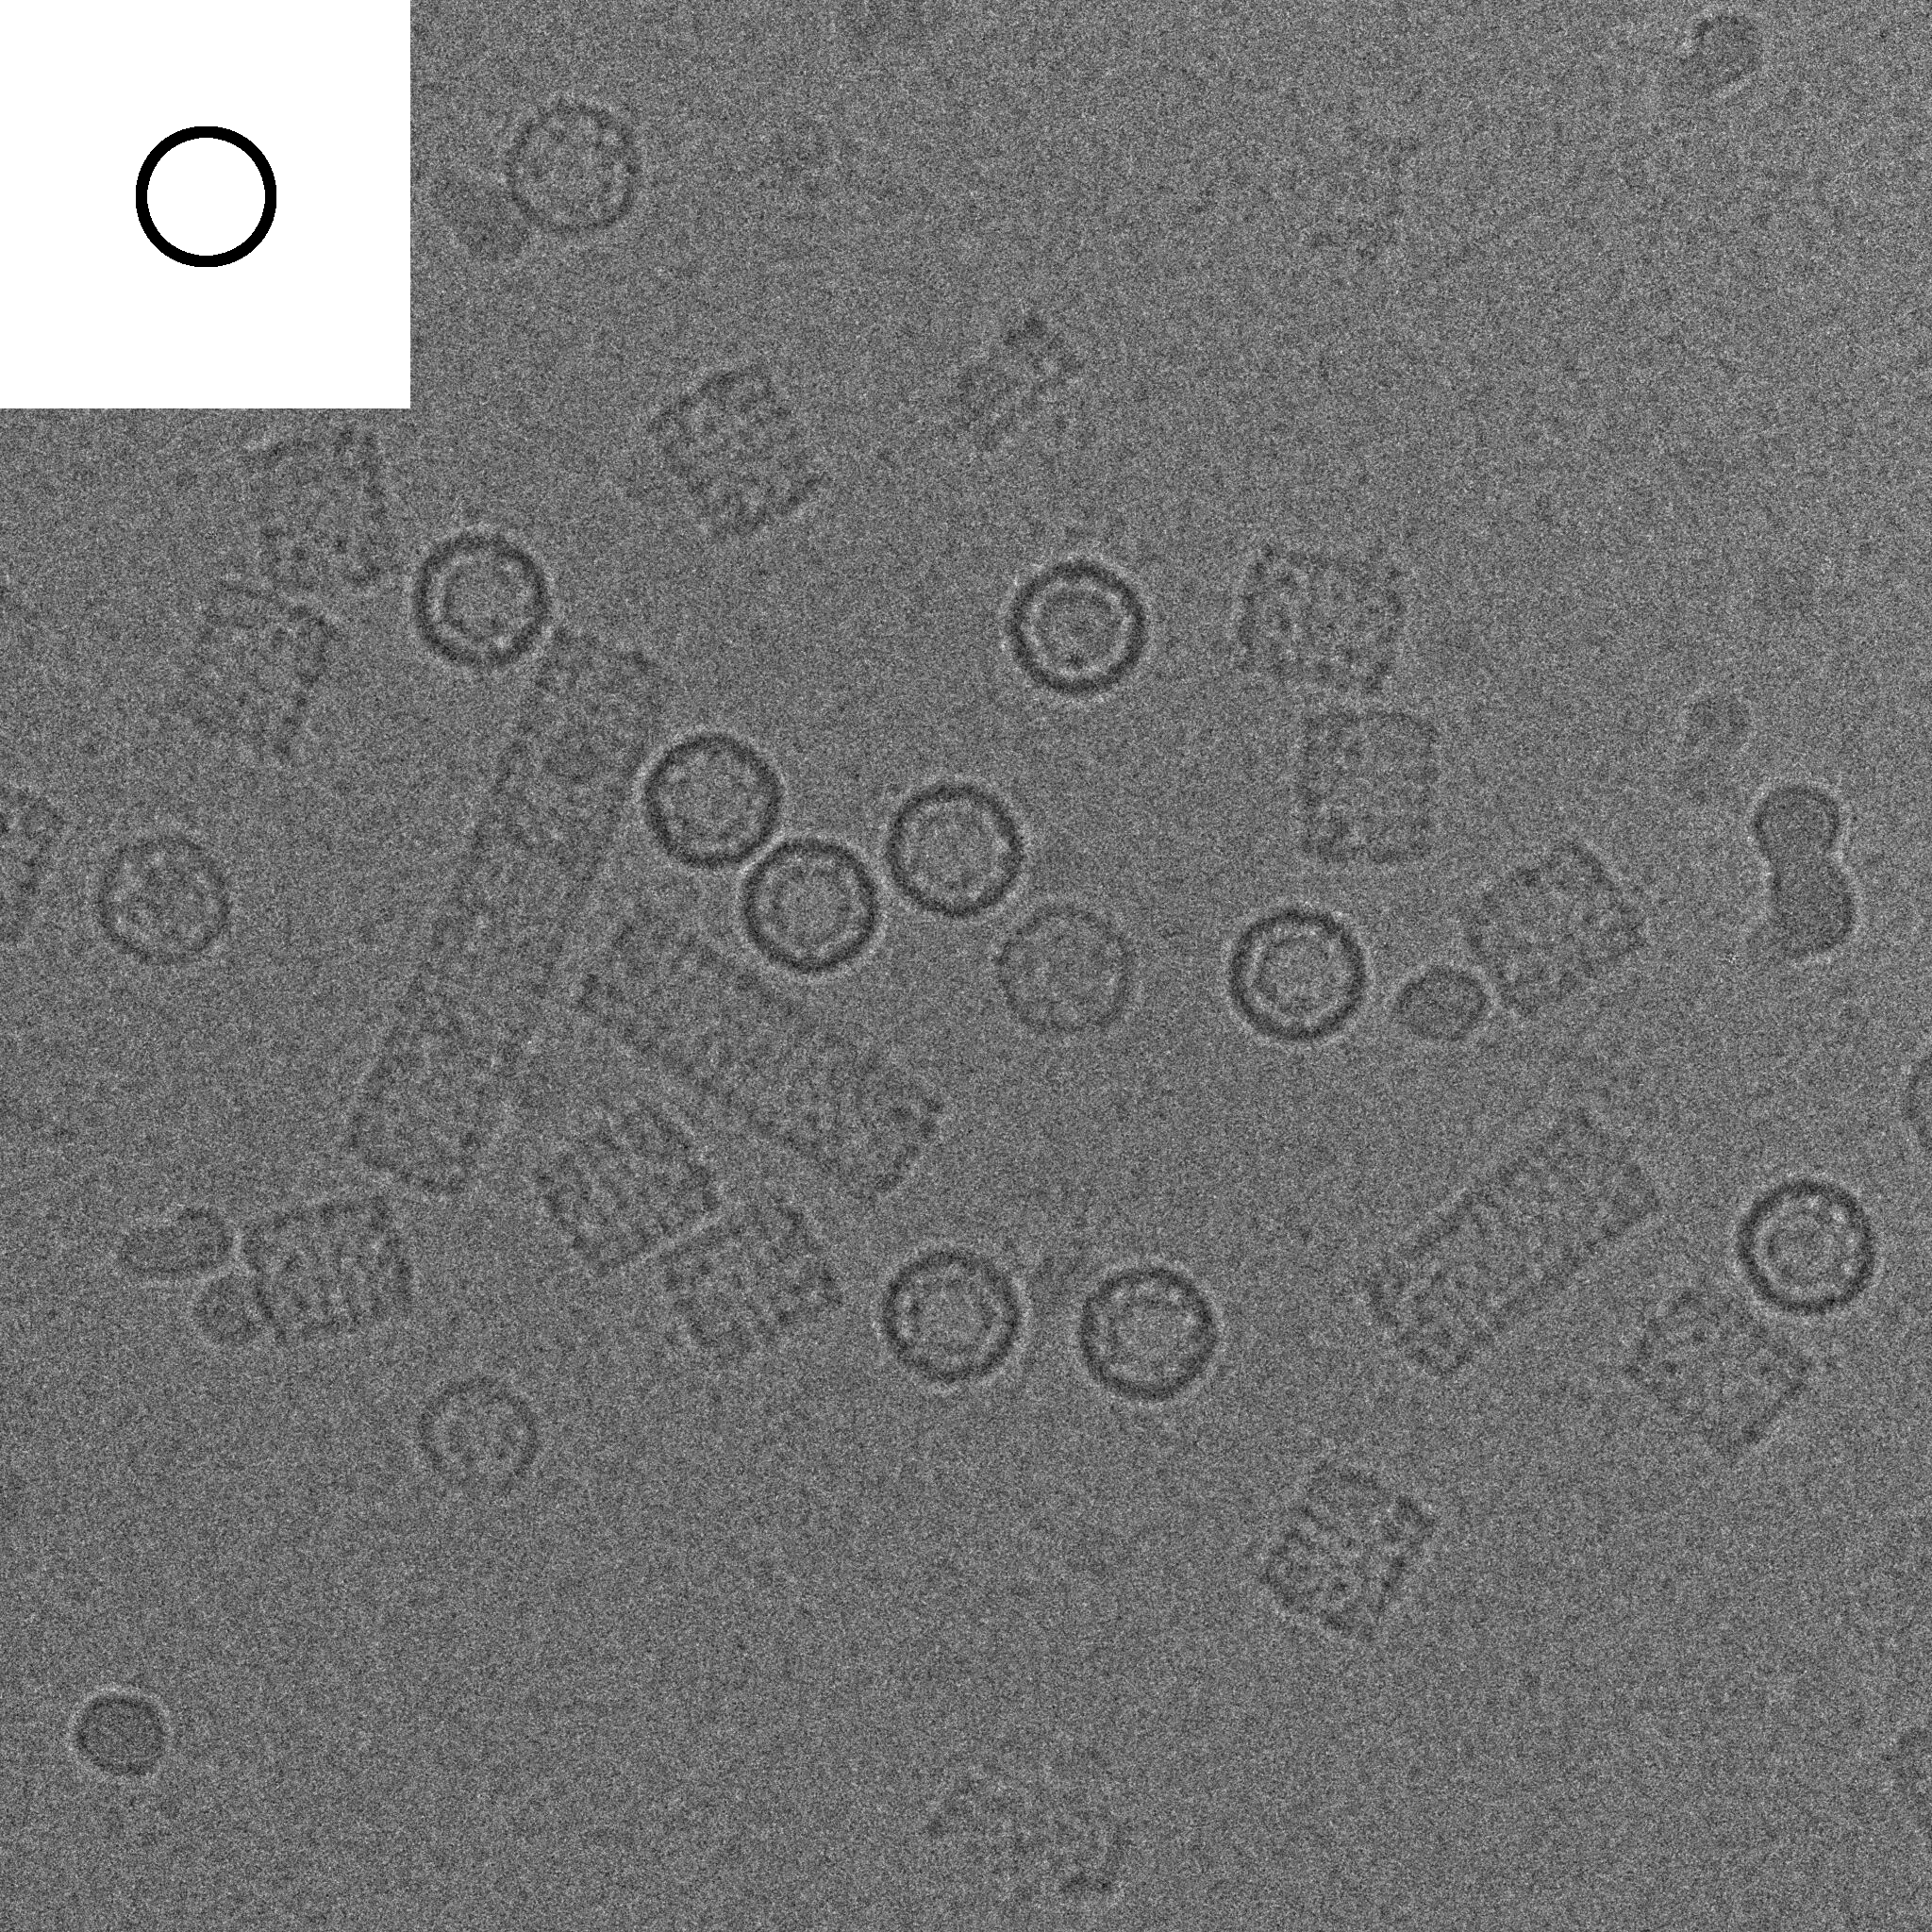
\includegraphics[scale=0.07]{exempleRond.png}
				
				Image pour la corrélation croisée avec la référence
			\end{figure}
				
		\end{column}
		\begin{column}{5cm}
			\begin{figure}
				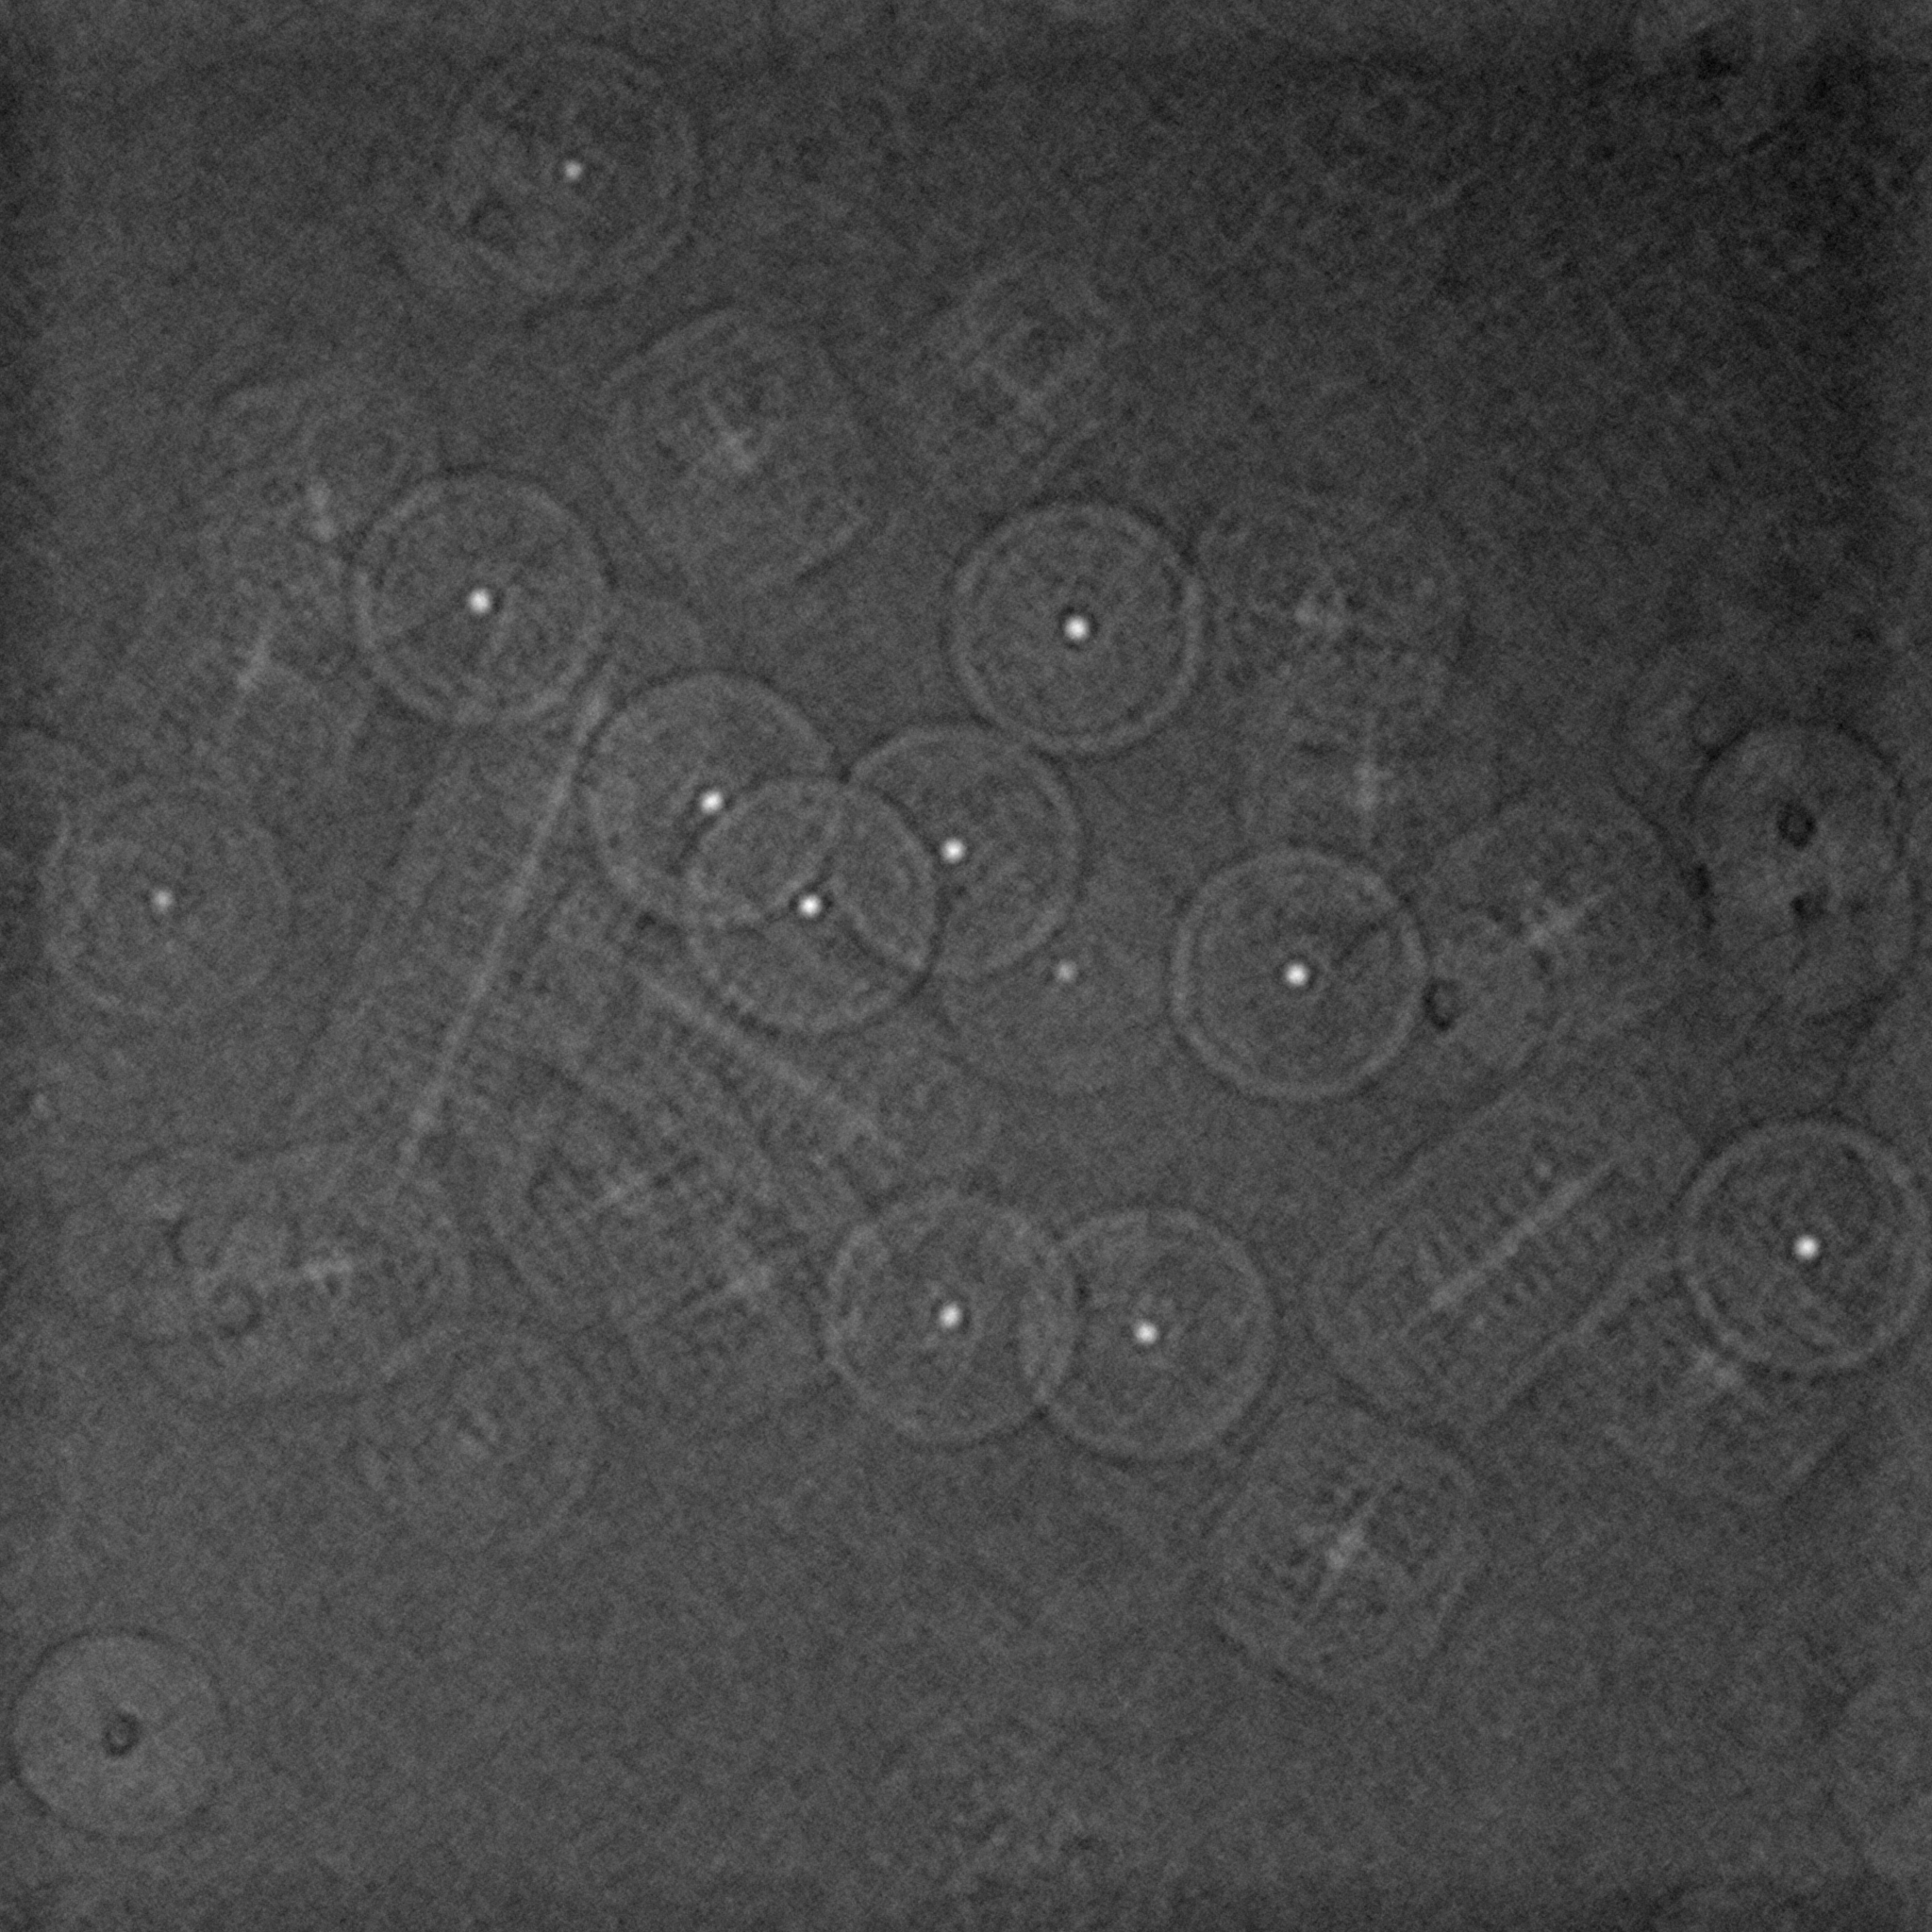
\includegraphics[scale=0.07]{Result.png}

				Image résultante
			\end{figure}
		\end{column}
	\end{columns}
\end{frame}

\subsubsection*{Démonstration avec DoG}

\begin{frame}
\frametitle{\subsubsecname}%
			\begin{figure}
				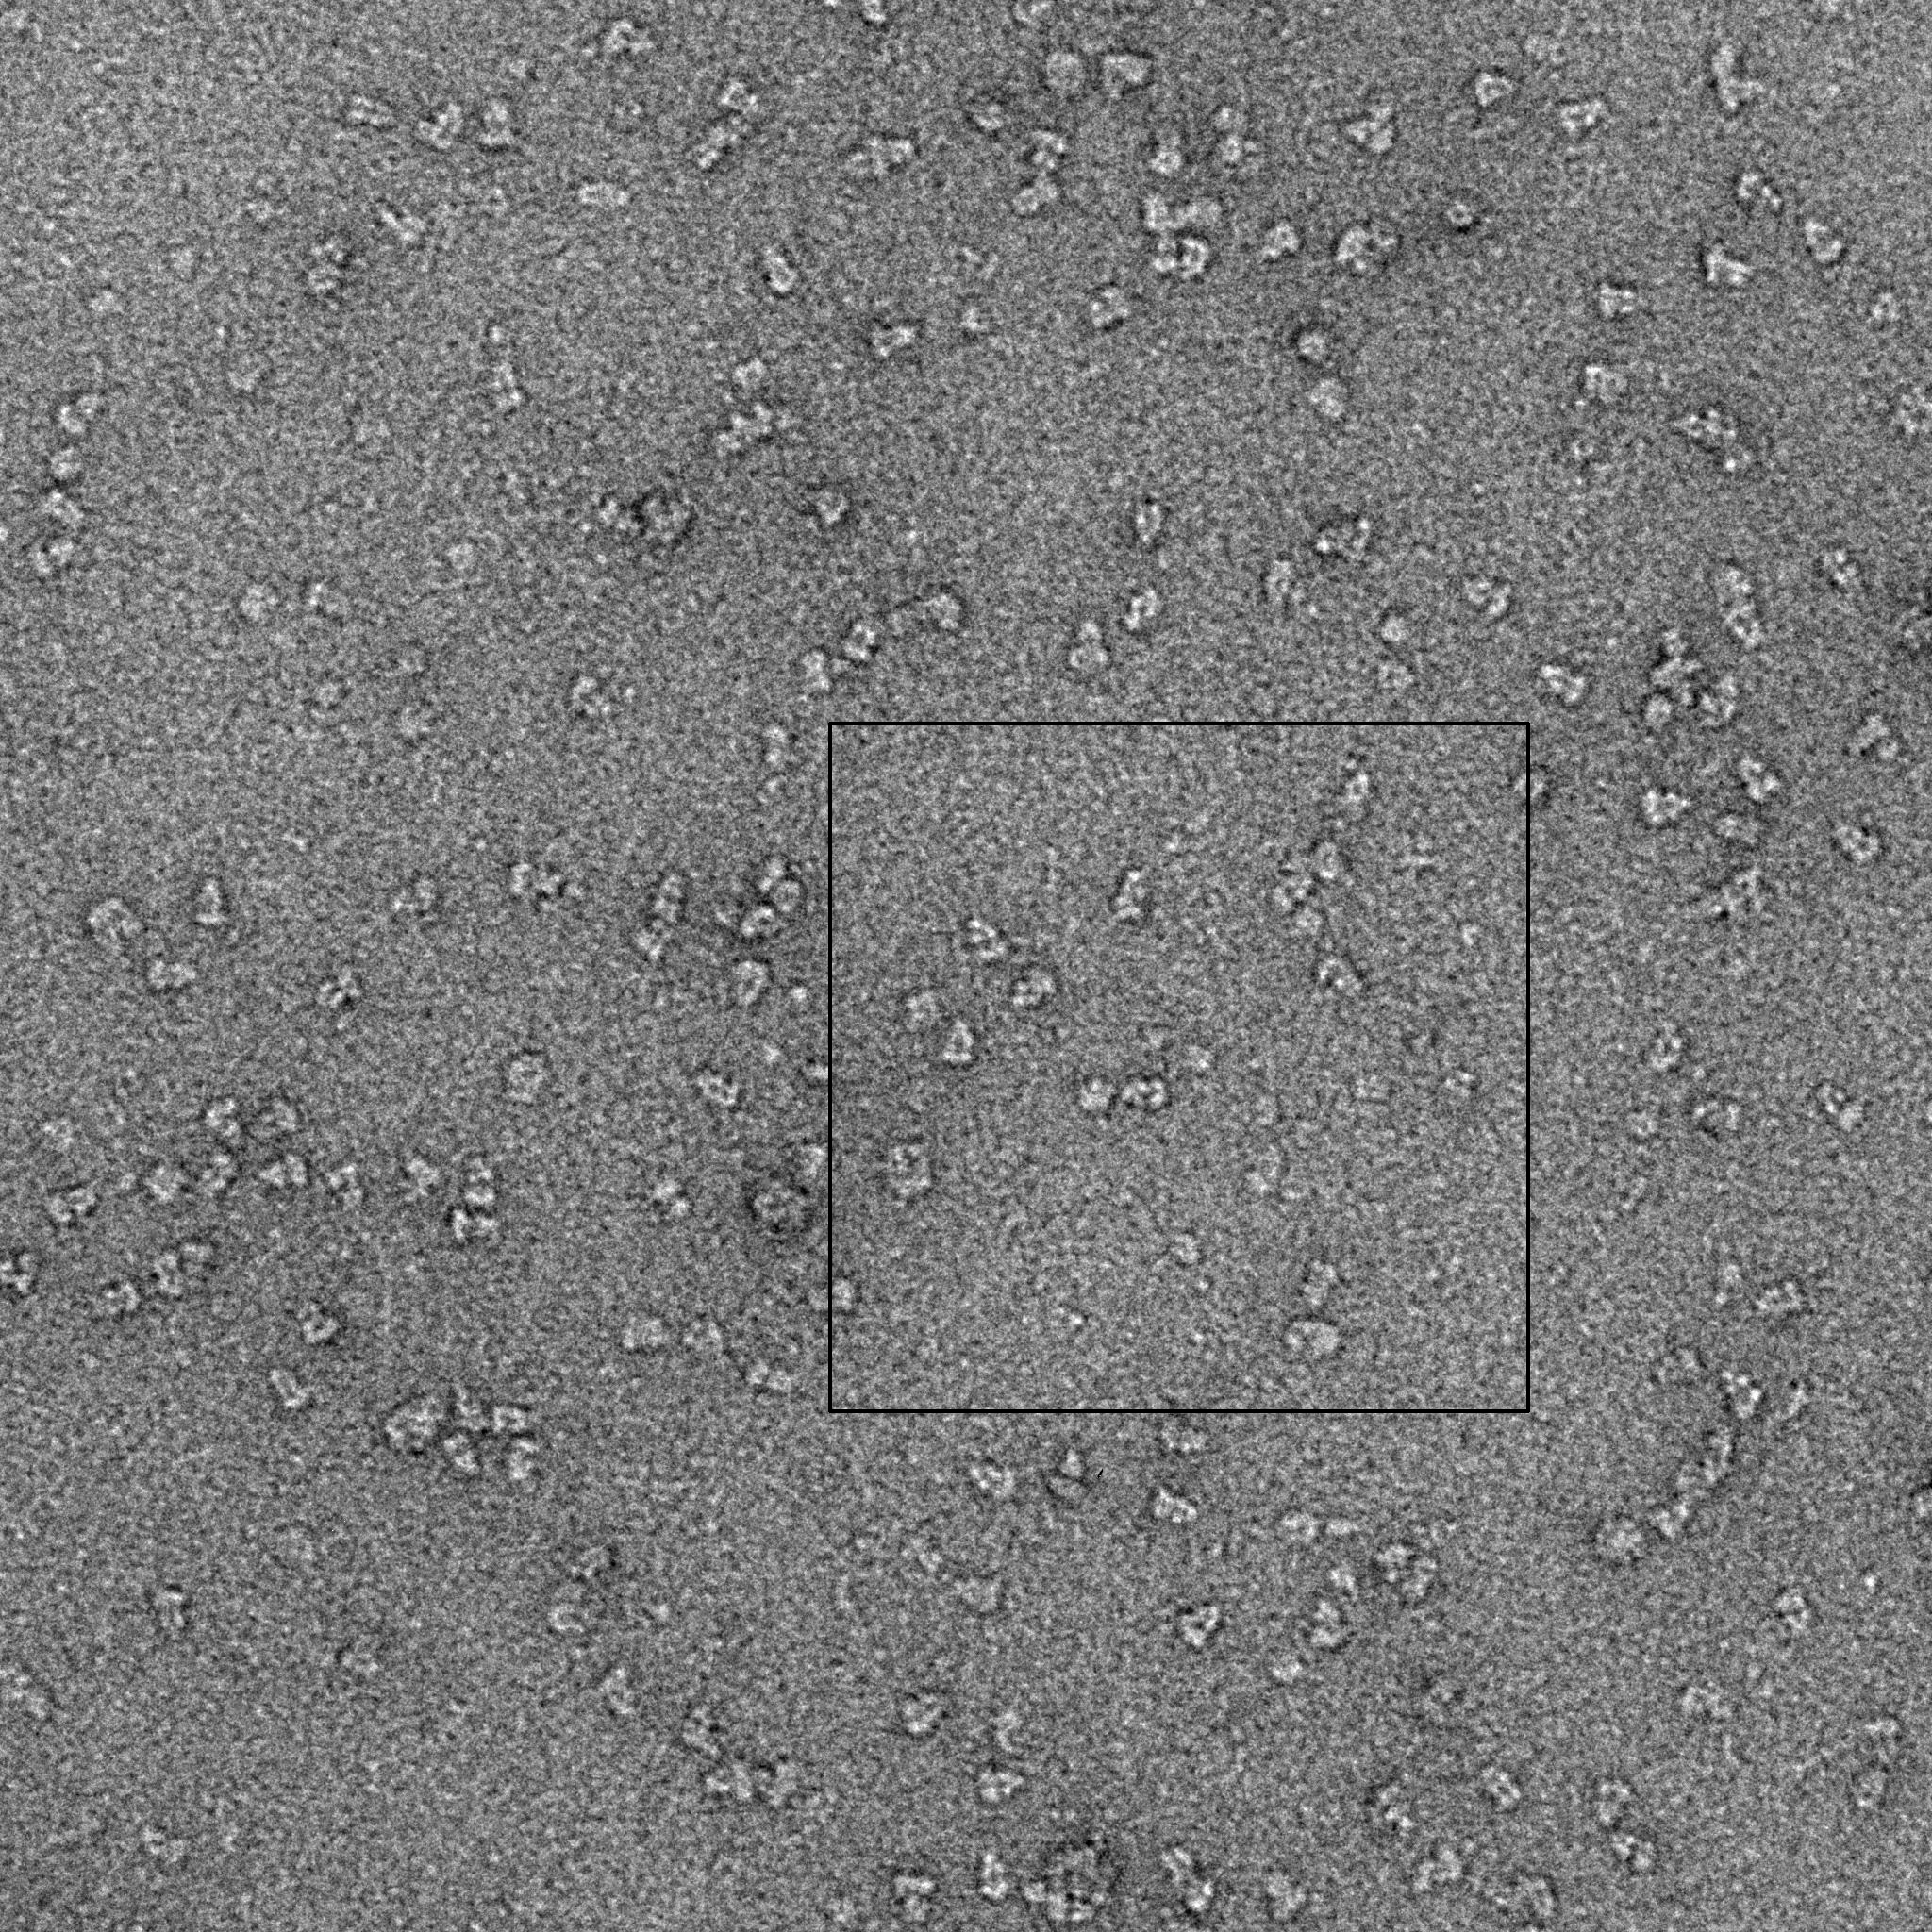
\includegraphics[scale=0.09]{base.png}
	
				Micrographie de protéines transmembranaires
			\end{figure}
\end{frame}

\begin{frame}
\frametitle{\subsecname ~- Les filtres}
	\begin{columns}
		\begin{column}{7cm}
			\begin{figure}
				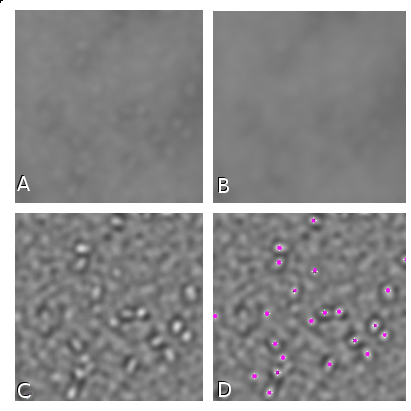
\includegraphics[scale=0.45]{Montage.png}
			\end{figure}
		\end{column}
		\begin{column}{5cm}
		A : Filtre Gaussien ($\sigma$ = 15)\\
		
		B : Filtre Gaussien ($\sigma$ = 20)\\

		C : Résultat de la soustraction \\

		D : Maxima locaux\\
		\end{column}
	\end{columns}
\end{frame}

\subsection{Résultats}

\begin{frame}
\frametitle{\subsecname} 
\begin{center}
Statistiques préliminaires de sélection \\
\end{center}
	\begin{table}[h]
	\begin{center}
	
	\begin{scriptsize}
	\begin{tabular}{|c|c|c|c|c|}
	\hline
	\textbf{Images} & \textbf{Variables} & \textbf{DoG} & \textbf{Extraction} & \textbf{Corrélation} \\
	\hline
	& Vrais Positifs  & 63 & 61 & X \\
	& Vrais Négatifs & 3 & 0 & X \\
Blobs & Faux Positifs & 9 & 2 & X \\
	& Faux Négatifs & 0 & 1 & X \\
	& Sensibilité & 1 & 0.98 & X \\
	& Spécificité & 0.25 & 0 & X \\
\hline
	& Vrais Positifs & 167 & X & X \\
	& Vrais Négatifs & 8 & X & X \\
Protéines Mb & Faux Positifs & 16 & X & X \\
	& Faux Négatifs & 8 & X & X \\
	& Sensibilité & 0.95 & X & X \\
	& Spécificité & 0.5 & X & X \\
	\hline
	& Vrais Positifs & 35 & X & 34 \\
	& Vrais Négatifs & 7 & X & 13 \\
Virus & Faux Positifs & 43 & X & 36 \\
	& Faux Négatifs & 2 & X & 3 \\
	& Sensibilité & 0.95 & X & 0.92 \\
	& Spécificité & 0.14 & X & 0.27 \\
	\hline
\end{tabular}
\end{scriptsize}
\end{center}
\end{table}
\end{frame}

\subsection{Difficultés et améliorations}

\begin{frame}
\frametitle{Difficultés rencontrées}
	\begin{block}{API ImageJ}
	Distinction :
		\begin{itemize}
			\item ImagePlus
			\item ImageProcessor
			\item ImageStack
		\end{itemize}
	\end{block}
	\begin{block}{GUI}
		\begin{itemize}
			\item Gestion des panneaux
			\item Organisation et tailles des fenêtres
		\end{itemize}
	\end{block}
\end{frame}

\begin{frame}
\frametitle{Améliorations 1/2}
	\begin{block}{Améliorer}
		\begin{itemize}
			\item Le mode Debug
			\item Continuer le travail pour l'utilisation en Macro
			\item Le post-traitement en fonction de la taille pour l'élimination des agrégats :
			\begin{itemize}
				\item Vérification visuelle
				\item Système d'apprentissage 
			\end{itemize}
		\end{itemize}
	\end{block}
	
\end{frame}

\begin{frame}
\frametitle{Améliorations 2/2}
	
		\begin{block}{Ajouter }
		
		\begin{itemize}
			\item Afficher les sélections pour chaque image d'une pile
			\item Contrôle visuel par l'opérateur
		\end{itemize}
		\end{block}
		\begin{columns}
			\begin{column}{5cm}
				\begin{figure}
					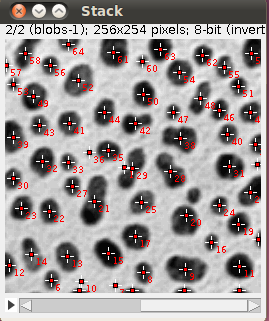
\includegraphics[scale=0.45]{BlobsOK.png}
				\end{figure}
			\end{column}
			\begin{column}{5cm}
				\begin{figure}
					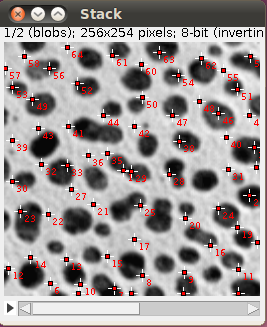
\includegraphics[scale=0.45]{BlobsPasOK-1.png}
				\end{figure}
			\end{column}
		\end{columns}
\end{frame}

\section{Conclusion}

\begin{frame}
\frametitle{\secname}
%Travail sympa, équipe cool, collègue parfois relou Taveau change tout le temps d'idée
	\begin{block}{Le projet}
		\begin{itemize}
			\item Interface facile d'utilisation
			\item Sélection efficace
			\item Récupération fonctionnelle des images individuelles et des coordonnées 
			\item Modularité pour l'ajout de nouveaux algorithmes
			\item Utilisation du logiciel \emph{Eclipse} et du gestionnaire de versions \emph{Git}
		\end{itemize}
	\end{block}
	\begin{block}{L'équipe}
		\begin{itemize}
			\item Première expérience de travail en équipe sur un gros projet concluante
			\item Aperçu de notre futur métier
		\end{itemize}
	\end{block}
\end{frame}
\begin{frame}
	\frametitle{}
	\begin{block}{}
		\begin{center}
			Merci beaucoup pour votre attention  %votez jean bon!
		\end{center}
	\end{block}
\end{frame}


\begin{frame}
\frametitle{Définitions}
\begin{itemize}

\item \textbf{Vrais Positifs} = particules devant être sélectionnées et qui le sont par l'algorithme \\
\item \textbf{Vrais Négatifs}  = tout ce qui ne doit pas être sélectionné et qui ne l'est pas \\
\item \textbf{Faux Positifs} = tout ce qui ne doit pas être sélectionné mais qui l'est \\
\item \textbf{Faux Négatifs} = particules devant être sélectionnées mais qui ne le sont pas \\ 
\item \textbf{Sensibilité} = probabilité qu'une particule devant être piquée le soit \\
\item \textbf{Spécificité} = probabilité de ne pas sélectionner ce qui ne doit pas l'être \\

\end{itemize}
\begin{center}
SE = $\frac{\text{VP}}{\text{VP+FN}}$ et SP = $\frac{\text{VN}}{\text{VN+FP}}$ \\
\end{center}
\end{frame}

\begin{frame}
\frametitle{Organisation d'une interface en Java}
\begin{figure}
	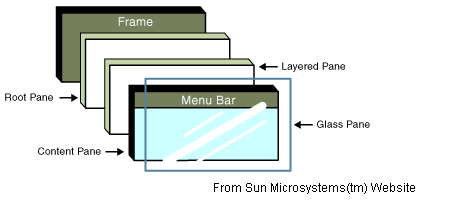
\includegraphics[scale=0.6]{Introduction_4.png}
	
	Exemple d'organisation de fenêtre
\end{figure}
\end{frame}

\end{document}